\documentclass[a4paper,12pt]{article}
\usepackage[utf8]{inputenc}
\usepackage[spanish]{babel}
\usepackage{graphicx}
\usepackage{libertine}
\usepackage{amsmath}
\renewcommand\familydefault{\sfdefault}
\usepackage[T1]{fontenc}
\usepackage[colorlinks=true,linkcolor=blue]{hyperref}
\usepackage[framed,numbered,autolinebreaks,useliterate]{mcode}

\parindent = 0mm

\author{Moisés Gautier Gómez}
\title{
\includegraphics[width=10cm]{logo_ugr.png} \\ 
\includegraphics[width=3cm]{fetch.png}\\ Práctica 5 - Teoría de la Señal y Comunicaciones 
}
\date{ }

\begin{document}
\maketitle
\tableofcontents
\clearpage
%\lstinputlisting{genexp.m}

\section{Ejercicio 1}
Para la ecuación en diferencias: $y(n)+0.9y(n-2) = 0.3x(n) + 0.6x(n-1) + 0.3x(n-2) $:\\

\textbf{a)} Calcule analíticamente $y(n)$ , para $x(n) = \delta (n)$.
Como la transformada Z de $x(\delta)$ es 1, la transformada de Z de Y es:
$$ Y(z) + 0,9 z^{-2} Y(z) = 0,3 X(z) + 0,6 z^{-1} X(z) + 0,3 z^{-2} X(z)$$
$$ Y(z)(1 + 0,9 z^{-2}) = X(z)(0,3 + 0,6 z^{-1} + 0,3 z^{-2})$$
$$ Y(z) = \frac{0,3 + 0,6 z^{-1} + 0,3 z^{-2}}{(1 + 0,9 z^{-2}) \cdot X(z)}$$
$$ X(z) = 1 $$
$$ Y(z) = \frac{(0,3 + 0,6 z^{-1} + 0,3 z^{-2})}{(1 + 0,9 z^{-2})}$$

Ahora descomponemos en fracciones simples el anterior resultado:
\begin{eqnarray*}
Y(z) & = & a + \frac{b + cz^{-1}}{(1 + 0,9z^{-2})} \\ & = & \frac{a \cdot (1 + 0,9z^{-2} + b + cz^{-1})}{(1 + 0,9z^{-2})} \\ & = & \frac{a + a 0,9 z^{-2} + b + cz^{-1}}{(1 + 0,9z^{-2})} \\ & = & \frac{(0,3 + 0,6z^{-1} + 0,3z^{-2})}{(1 + 0,9 z^{-2})}
\end{eqnarray*}

$$c = \frac{6}{10} $$
$$a = \frac{0,3}{0,9} = \frac{1}{3} $$
$$a + b = \frac{3}{10} \rightarrow b = \frac{3}{10} - \frac{1}{3} = - \frac{1}{30} $$

\begin{eqnarray*}
Y(z) & = & \frac{1}{3} + \frac{- \frac{1}{30} + \frac{6}{10}z^{-1}}{(1 + 0,9 z^{-2})} \\ & = & \frac{1}{3} + \frac{- \frac{1}{30} + \frac{6}{10}z^{-1}}{(1 - (-0,9) z^{-2})} \\ & = & \frac{1}{3} + \frac{- \frac{1}{30} + \frac{6}{10}z^{-1}}{(1 - \sqrt{-0,9} z^{-1})(1 + \sqrt{-0,9} z^{-1})}
\end{eqnarray*}

$$ \frac{A}{(1 - \sqrt{-0,9} z^{-1})} + \frac{B}{(1 + \sqrt{-0,9} z^{-1})} = \frac{- \frac{1}{30} + \frac{6}{10}z^{-1}}{(1 - \sqrt{-0,9} z^{-1})(1 + \sqrt{-0,9} z^{-1})} $$

$$ A(1 + (\sqrt{-0,9}) z^{-1}) + B(1 - (\sqrt{-0,9}) z^{-1}) = - \frac{1}{30} + \frac{6}{10} z^{-1}$$
$$ A + A \sqrt{-0,9} z^{-1} + B - B\sqrt{-0,9} z^{-1} = - \frac{1}{30} + \frac{6}{10} z^{-1}$$
$$ A + B = - \frac{1}{30}, A\sqrt{-0,9} - B\sqrt{-0,9} = \frac{6}{10} $$
$$ A + B = - \frac{1}{30}, A - B = \frac{6}{10 \sqrt{-0,9}} $$
$$ A + B = - \frac{1}{30}, A - B = \frac{-2 \sqrt{-0,9}}{3} $$
$$ A = -  \frac{1}{60} - \frac{i \sqrt{0,9}}{3} $$
$$ B = -  \frac{1}{60} + \frac{i \sqrt{0,9}}{3} $$
$$ Y(z) = \frac{1}{3} + \frac{-\frac{1}{60} - \frac{i \sqrt{0,9}}{3}}{(1 - (\sqrt{-0,9}) z^{-1})} + \frac{-\frac{1}{60} + \frac{i \sqrt{0,9}}{3}}{(1 + (\sqrt{-0,9}) z^{-1})}$$

Por último calculamos la inversa según las tablas:

$$ y(n) = \frac{1}{3} \delta(n) + (- \frac{1}{60} - \frac{i \sqrt{0,9}}{3})(i \sqrt{0,9})^n u(n) + (- \frac{1}{60} + \frac{i \sqrt{0,9}}{3})(-i \sqrt{0,9})^n u(n)$$

\textbf{b)} Cree un vector impulso unidad de longitud 128. Genere los 128 primeros valores de la respuesta al impulso del filtro y represente gráficamente los valores obtenidos. \\
\begin{center}
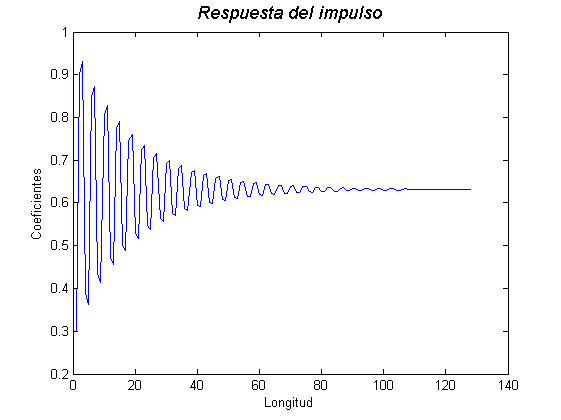
\includegraphics[width=.8 \textwidth]{ejercicio1-b.png}
\end{center}

\textbf{c)} Determine la función de transferencia; determine sus polos y sus ceros y represéntelos gráficamente. Justifique la estabilidad del sistema. \\

Función de transferencia:
\begin{eqnarray*}
H(z) & = & \frac{Y(z)}{X(z)} = \frac{0,3 + 0,6 z^{-1} + 0,3 z^{-2}}{1 + 0,9 z^{-2}} \\ & = & \frac{0,3 (1 + 2 z^{-1} + z^{-2})}{(1 - \sqrt{-0,9} z^{-1})(1 + \sqrt{-0,9} z^{-1})} \\ & = & \frac{0,3 (1 + z^{-1})^2}{(1 - \sqrt{-0,9} z^{-1})(1 + \sqrt{-0,9} z^{-1})}
\end{eqnarray*}

Polos: $z = \pm i \sqrt{0,9}$ \\

Ceros: $z = -1$ \\

Representación: \\
\begin{center}
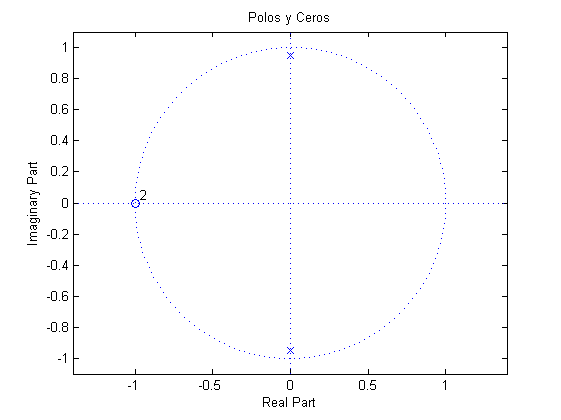
\includegraphics[width=.8 \textwidth]{polos-ceros-ejercicio1.png}
\end{center}

Como los valores de los tiempos positivos son distintos de 0, entonces el sistema es causal. Para que converja a un valor: $ |z| > \pm i \sqrt{0,9} $ \\

La Rdc (Región de convergencia) es la zona del plano que esta fuera del círculo de radio $\sqrt{0,9}$, por tanto, la Rdc incluye al círculo unidad y el sistema es estable. \\

Aquí muestro el código Matlab asociado:\\
\lstinputlisting{ejercicio1.m}

\section{Ejercicio 2}
Respuesta al escalón. Para el sistema anterior obtenga la respuesta a un escalón de amplitud 3.\\

\textbf{a)} Represente la función escalón y determine el nivel constante de salida cuando n tiende a infinito. Este nivel constante determinado es la Respuesta en régimen permanente. \\

\begin{center}
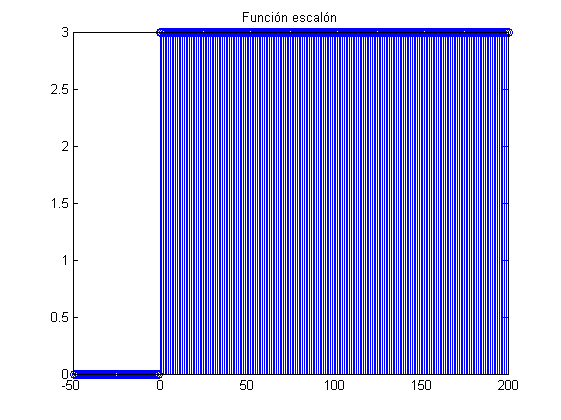
\includegraphics[width=.8 \textwidth]{funcion-escalon-ejercicio-2.png}\\
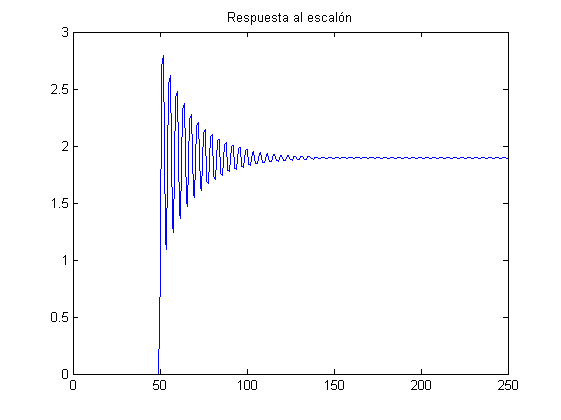
\includegraphics[width=.8 \textwidth]{respuesta-impulso-funcion-escalon-ejercicio-2.png}
\end{center}

Respuesta en régimen permanente: 1,895\\

\textbf{b)} La parte variable de la respuesta total es la Respuesta transitoria. Determine la respuesta transitoria (reste a la respuesta al escalón el valor constante de salida). \\

\begin{center}
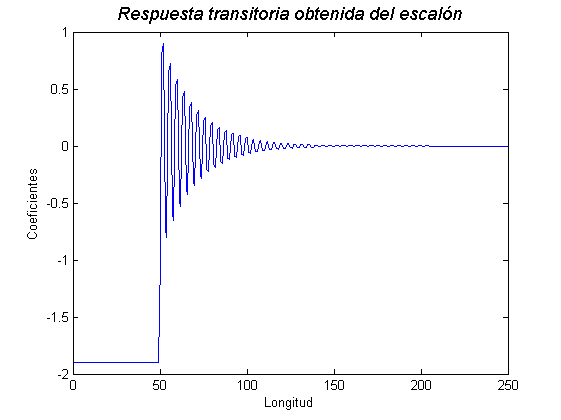
\includegraphics[width=.8 \textwidth]{respuesta-transitoria-al-escalon-ejercicio-2.png}
\end{center}

\textbf{c)} Represente gráficamente la respuesta transitoria en el intervalo $0 \leq n \leq 50$.

\begin{center}
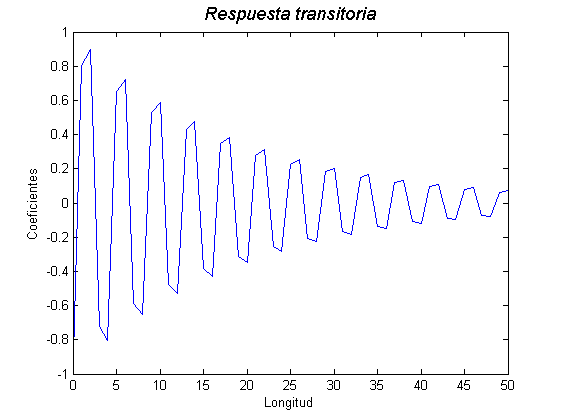
\includegraphics[width=.8 \textwidth]{respuesta-transitoria-ejercicio-2.png}
\end{center}

Aquí muestro el código Matlab asociado:\\
\lstinputlisting{ejercicio2.m}

\section{Ejercicio 3}

Para la ecuación en diferencias anterior realice los siguientes cálculos usando \textbf{freqz}. \\

\textbf{a)} Represente la gráfica módulo y fase con 512 muestras de frecuencias alrededor de toda la circunferencia unidad. \\

\begin{center}
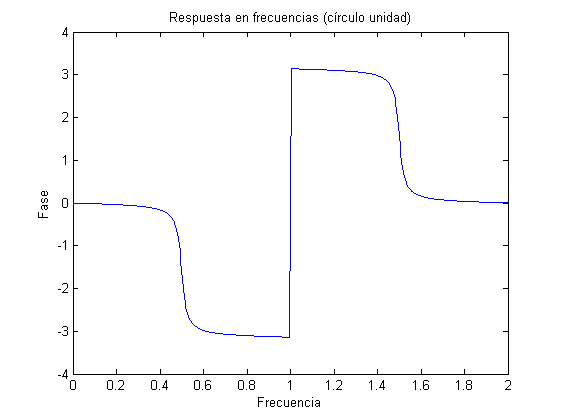
\includegraphics[width=.8 \textwidth]{respuesta-frecuencias-unidad-fase-ejercicio-3.png}
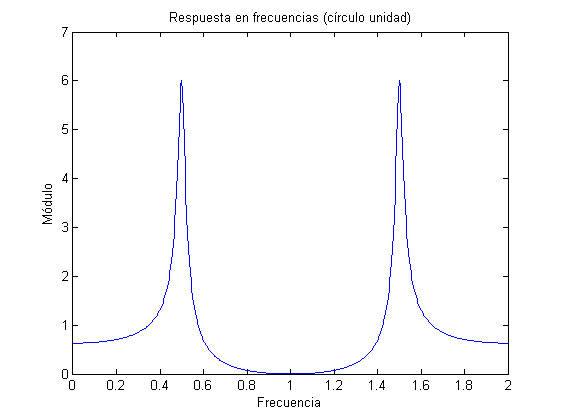
\includegraphics[width=.8 \textwidth]{respuesta-frecuencias-unidad-modulo-ejercicio-3.png}
\end{center}

\textbf{b)} Realice la misma representación utilizando únicamente la mitad superior de la circunferencia de radio unidad. \\

\begin{center}
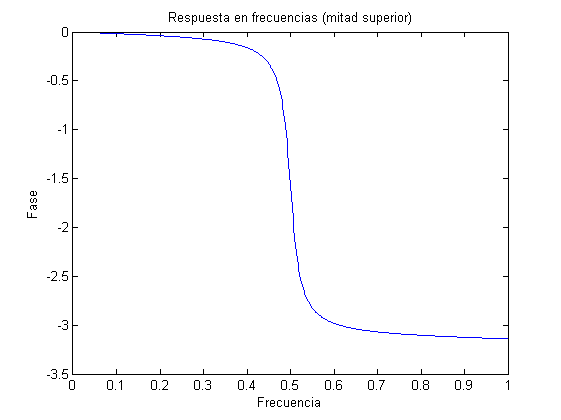
\includegraphics[width=.8 \textwidth]{respuesta-frecuencias-unidad-fase-mitad-ejercicio-3.png}
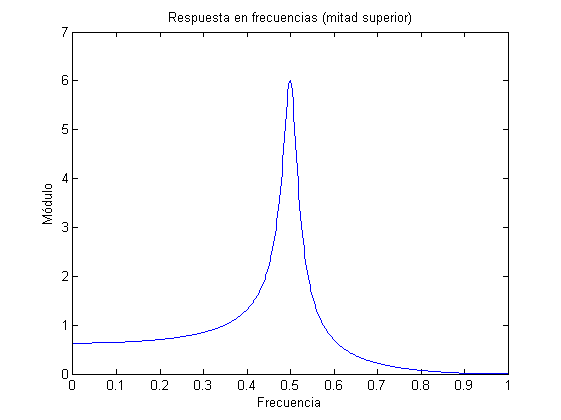
\includegraphics[width=.8 \textwidth]{respuesta-frecuencias-unidad-modulo-mitad-ejercicio-3.png}
\end{center}

\textbf{c)} Comente el tipo de filtro definido por esta ecuación en diferencias. \\

Es un filtro paso banda, que solo deja pasar las frecuencias con valores entre $\frac{\pi}{2}$ y $\frac{3 \pi}{2}$.\\

Aquí muestro el código Matlab asociado:\\
\lstinputlisting{ejercicio3.m}

\section{Ejercicio 4}

Repita los pasos 1, 2 y 3 con las siguientes ecuaciones en diferencias: \\

\textbf{a)} $y(n) + 0,13y(n-1) + 0,2y(n-2) + 0,3y(n-3) = 0,6 x(n) - 0,48 x(n-1) + 0,48 x(n-2) - 1,6 x(n-3)$\\

\textbf{1.a)}\\

Calculamos la transformada $Z$ de $Y$.
\begin{eqnarray*}
Y(z) & + & 0,13 z^{-1} Y(z) + 0,2 z^{-2} Y(z) + 0,3 z^{-3} Y(z) \\ & = & 0,6 X(z) - 0,48 z^{-1} X(z) + 0,48 z^{-2} X(z) - 1,6 z^{-3} X(z)
\end{eqnarray*}
$$ Y(z) = \frac{(0,6 - 0,48 z^{-1} + 0,48 z^{-2} - 1,6 z^{-3})}{(1 + 0,13 z^{-1} + 0,2 z^{-2} + 0,3 z^{-3})}$$

Descomponemos en fracciones simples. Como calcular las raíces es bastante complicado, por ello utilizaremos directamente la función residuez para hallar la descomposición:

\lstinputlisting{ejercicio-4-1-a.m}

$$ r = 1,4005 - 0,5153i; 1,4005 + 0,5153i; 3,1323 $$
$$ p = 0,2397 + 0,6594i; 0,2397 - 0,6594i; -0,6095 $$
$$ k = -5,3333 $$

Por lo que la ecuación queda como sigue:

\begin{eqnarray*}
Y(z) & = & \frac{1,4005 - 0,5153i}{(1 - (0,2397 + 0,6594 i) z^{-1})} \\ & + & \frac{1,4005 + 0,5153i}{(1 - (0,2397 - 0,6594 i) z^{-1})} \\ & + & \frac{3,1323}{(1 - (-0,6095) z^{-1})} - 5,3333
\end{eqnarray*}

Calculamos la inversa según las tablas: 

\begin{eqnarray*}
y(n) & = & (1,4005 - 0,5153 i)(0,2397 + 0,6594i)^n u(n) \\ & + & (1,4005 + 0,5153i)(0,2397 - 0,6594i)^n u(n) \\ & + & 3,1323 (-0,6095)^n u(n) - 5,3333 \delta(n)
\end{eqnarray*}

\textbf{1.b)} \\

\begin{center}
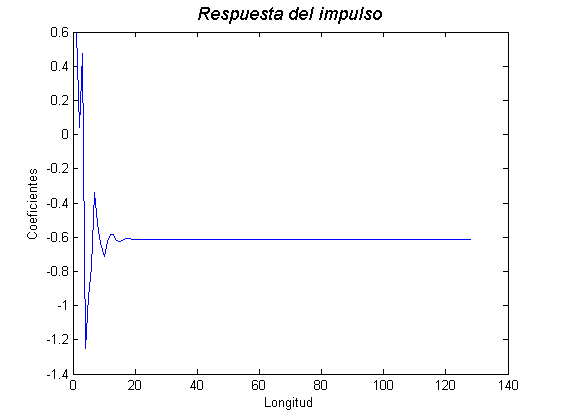
\includegraphics[width=.8 \textwidth]{ejercicio-4-1-b.png}
\end{center}

\textbf{1.c)} \\

$$ Y(z) = \frac{(0,6 - 0,48 z^{-1} + 0,48 z^{-2} - 1,6 z^{-3})}{(1 + 0,13 z^{-1} + 0,2 z^{-2} + 0,3 z^{-3})}$$

Polos: $ 1 + 0,13 z^{-1} + 0,2 z^{-2} + 0,3 z^{-3} = 0 $ (Lo resolvemos mediante solve) \\
$$ -0,6095;\ 0,2397 - 0,6594i;\ 0,2397 + 0,6594i $$
Ceros: $ 0,6 - 0,48 z^{-1} + 0,48 z^{-2} -1,6 z^{-3} = 0 $ \\
$$ 1,4786;\ -0,3393 - 1,2994i;\ -0,3393 + 1,2994i $$

\lstinputlisting{solve-1.m}

Representación: \\

\begin{center}
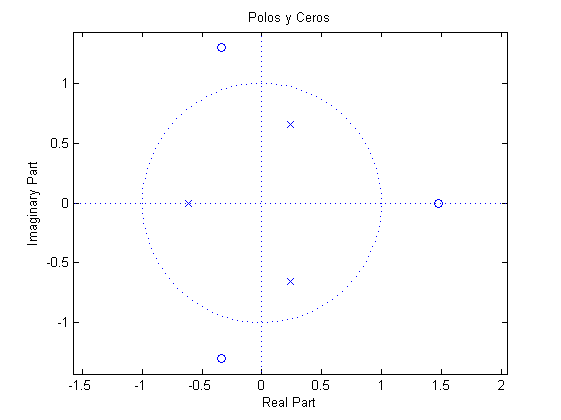
\includegraphics[width=.8 \textwidth]{ejercicio-4-1-c.png}
\end{center}

Como el sistema es causal, $|z| > polos$. Todos los polos son menores que 1 en módulo, por lo que la Rdc será la parte del plano mayor que el círculo de radio 0,6594. Por lo tanto, el círculo unitario está dentro de esta zona, y el sistema es estable. \\

Aquí muestro el código Matlab para los apartados b) y c):\\

\lstinputlisting{ejercicio-4-1-b.m}

\textbf{2.a)}\\

\begin{center}
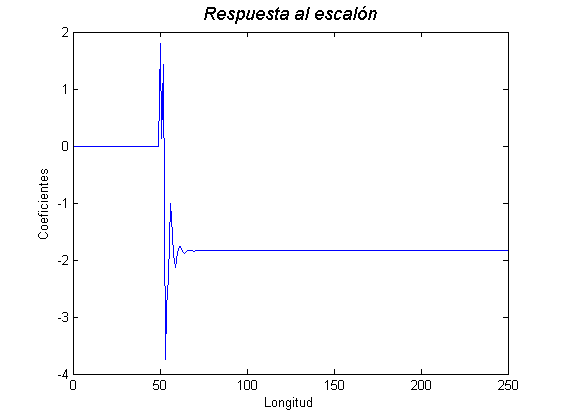
\includegraphics[width=.8 \textwidth]{ejercicio-4-2-a.png}
\end{center}

Respuesta en régimen permanente: -1,8405 \\

\lstinputlisting{ejercicio-4-2-a.m}

\textbf{2.b)}\\

\begin{center}
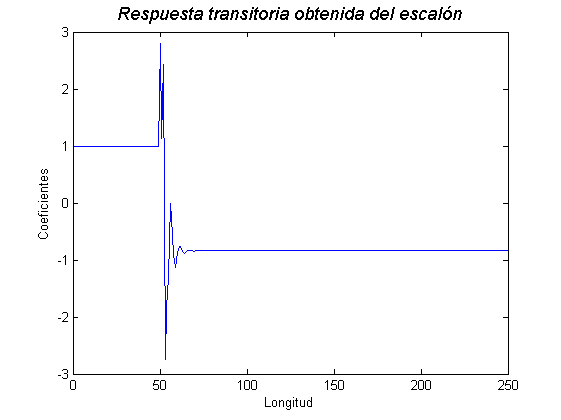
\includegraphics[width=.8 \textwidth]{ejercicio-4-2-b.png}
\end{center}

\lstinputlisting{ejercicio-4-2-b.m}

\textbf{2.c)}\\

\begin{center}
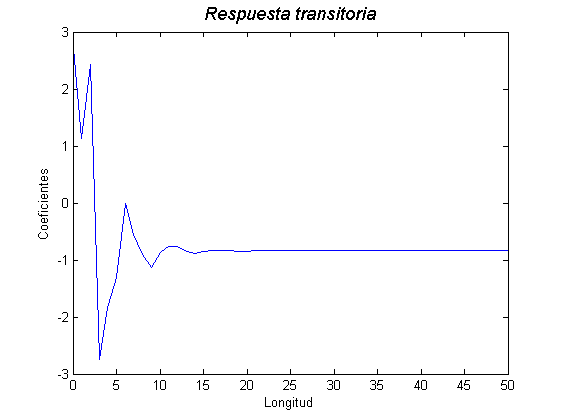
\includegraphics[width=.8 \textwidth]{ejercicio-4-2-c.png}
\end{center}

\lstinputlisting{ejercicio-4-2-c.m}

\textbf{3.a)}\\

\begin{center}
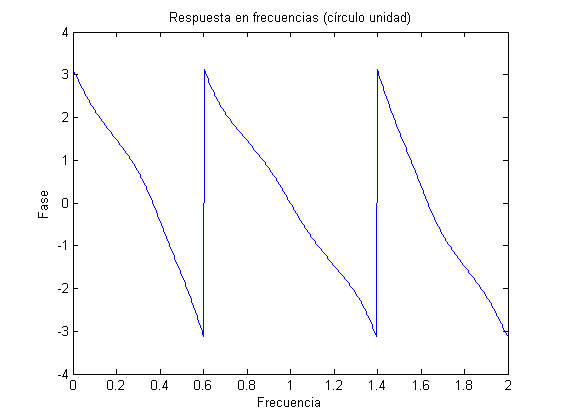
\includegraphics[width=.8 \textwidth]{ejercicio-4-3-a-fase.png}\\
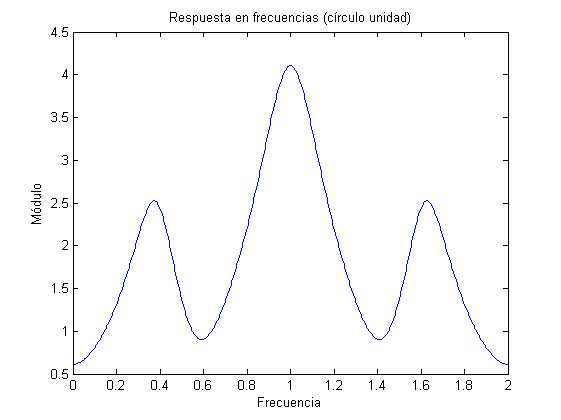
\includegraphics[width=.8 \textwidth]{ejercicio-4-3-a-modulo.png}
\end{center}

\textbf{3.b)}\\

\begin{center}
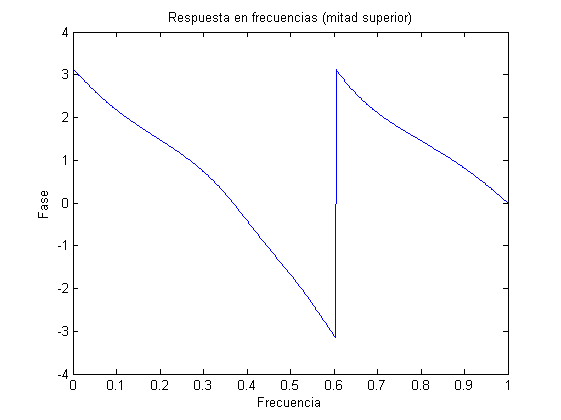
\includegraphics[width=.8 \textwidth]{ejercicio-4-3-b-fase.png}\\
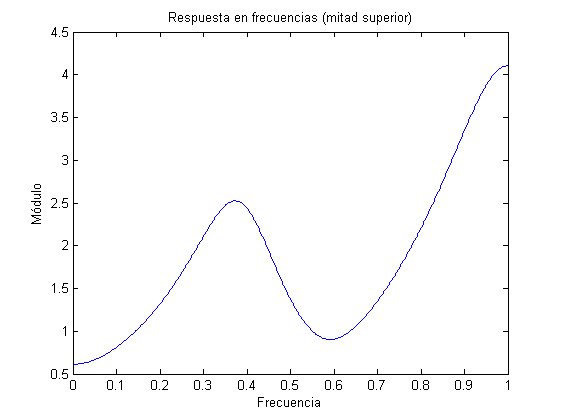
\includegraphics[width=.8 \textwidth]{ejercicio-4-3-b-modulo.png}
\end{center}

\textbf{3.c)}\\

Este filtro es un filtro paso banda que deja pasar alrededor de $0,6 \pi$ y $1,4 \pi$, mientras que no deja pasar las bajas frecuencias.

\lstinputlisting{ejercicio-4-3.m}

\textbf{b)} $10 y(n) - 5 y(n-1) + y(n-2) = x(n) - 5 x(n-1) + 10 x(n-2)$ \\

Realizamos los mismos cálculos pero cambiando los vectores de coeficientes:

$ a = [10 -5 1] $
$ b = [1 -5 10] $

\textbf{1.a)}

Calculamos la transformada de Z de Y. \\

\begin{eqnarray*}
10 Y(z) - 5 z^{-1} Y(z) + z^{-2Y(z)} & = & X(z) - 5 z^{-1} X(z) + 10 z^{-2} X(z) \\ & \rightarrow & Y(z) = \frac{(1 - 5 z^{-1} + 10 z^{-2})}{10 - 5 z^{-1} + z^{-2}}
\end{eqnarray*}

Descomponemos en fracciones simples. Como calcular las raíces es bastante complicado, utilizaremos directamente la función residuez para hallar la descomposición de las mismas: \\

\lstinputlisting{ejercicio-4-4-a.m}

$$ r = -4,9500 - 5,2285i; -4,9500 + 5,2285i; $$
$$ p = 0,2500 + 0,1936i; 0,2500 - 0,1936i; $$
$$ k = 10 $$

Por lo que la ecuación queda: \\

$$ Y(z) = \frac{-4,9500 - 5,2285i}{(1 - (0,2500 + 0,1936i)z^{-1})} + \frac{-4,9500 - 5,2285i}{(1 - (0,2500 + 0,1936i)z^{-1})} + 10 $$

Calculamos la inversa según las tablas:

\begin{eqnarray*}
y(n) & = & (-4,9500 - 5,2285i)(0,2500 + 0,1936i)^n u(n) \\ & + & (-4,9500 - 5,2285i)(0,2500 + 0,1936i)^n u(n) + 10 \delta(n)
\end{eqnarray*}

\textbf{1.b)} \\

\begin{center}
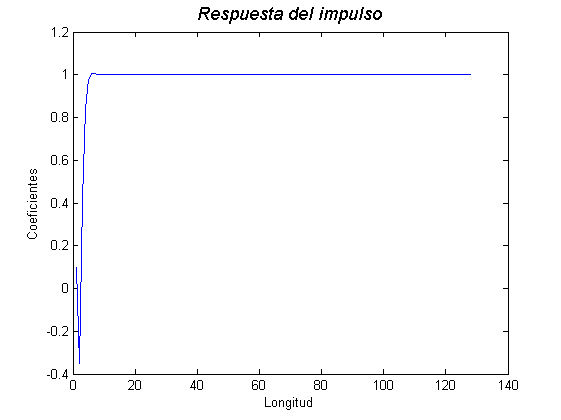
\includegraphics[width=.8 \textwidth]{ejercicio-4-4-b.png}
\end{center}

\textbf{1.c)} \\

$$ H(z) = \frac{(1 - 5 z^{-1} + 10 z^{-2})}{(10 - 5 z^{-1} + z^{-2})}$$

Polos: $ 10 - 5 z^{-1} + z^{-2} = 0 $ \\
$$ \frac{1}{4} \pm \frac{(15^{\frac{1}{2}} i)}{20}$$

Ceros: $ 1 - 5 z^{-1} + 10 z^{-2} = 0 $ \\
$$ \frac{5}{2} \pm \frac{(15^{\frac{1}{2}} i)}{2}$$

\lstinputlisting{solve-2.m}

Representación: \\

\begin{center}
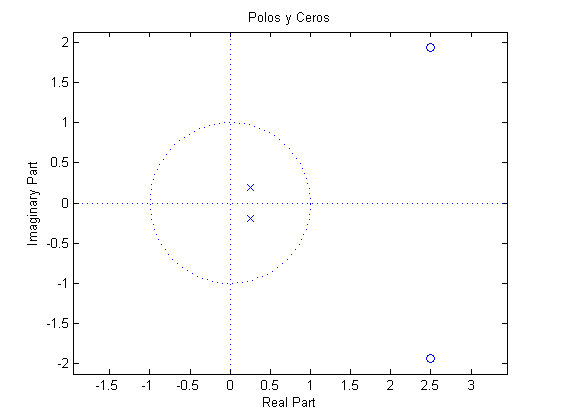
\includegraphics[width=.8 \textwidth]{ejercicio-4-4-b-polos.png}
\end{center}

Como el sistema es causal, $|z| > polos$. Todos los polos son menores que 1 en módulo, por lo que la Rdc será la parte del plano mayor que el círculo de radio 0,25. Así pues, el círculo unitario está dentro de esta zona, y el sistema es estable. \\

\lstinputlisting{ejercicio-4-4-b.m}

\textbf{2.a)} \\

\begin{center}
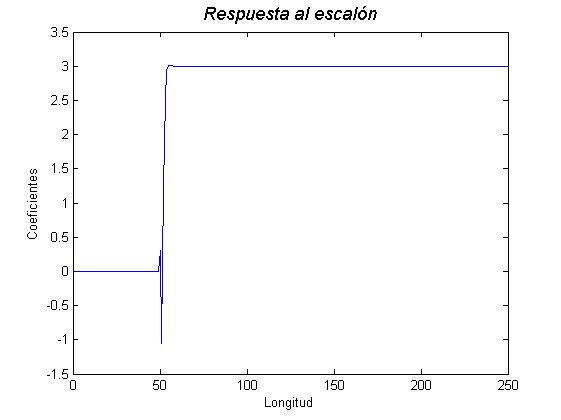
\includegraphics[width=.8 \textwidth]{ejercicio-4-5-a.png}
\end{center}

Respuesta en régimen permanente: 3.\\

\lstinputlisting{ejercicio-4-5-a.m}

\textbf{2.b)} \\

\begin{center}
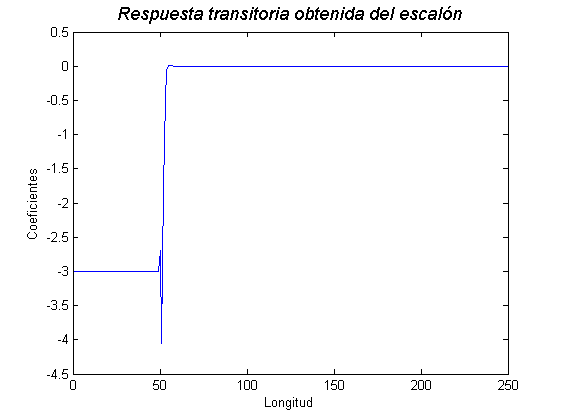
\includegraphics[width=.8 \textwidth]{ejercicio-4-5-b.png}
\end{center}

\lstinputlisting{ejercicio-4-5-b.m}

\textbf{2.c)} \\

\begin{center}
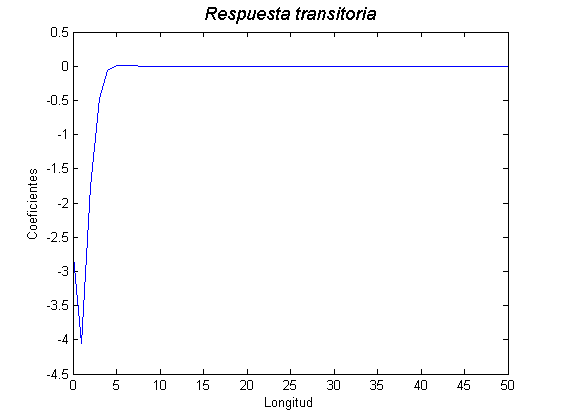
\includegraphics[width=.8 \textwidth]{ejercicio-4-5-c.png}
\end{center}

\lstinputlisting{ejercicio-4-5-c.m}

\textbf{3.a)} \\

\begin{center}
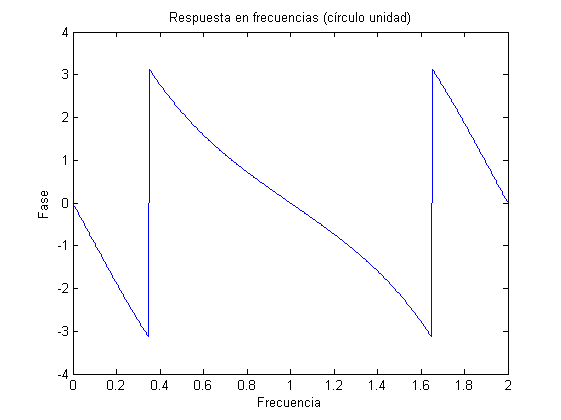
\includegraphics[width=.8 \textwidth]{ejercicio-4-6-a-fase.png}
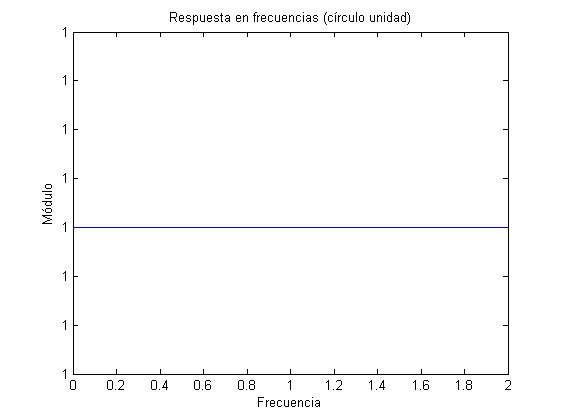
\includegraphics[width=.8 \textwidth]{ejercicio-4-6-a-modulo.png}
\end{center}

\textbf{3.b)} \\

\begin{center}
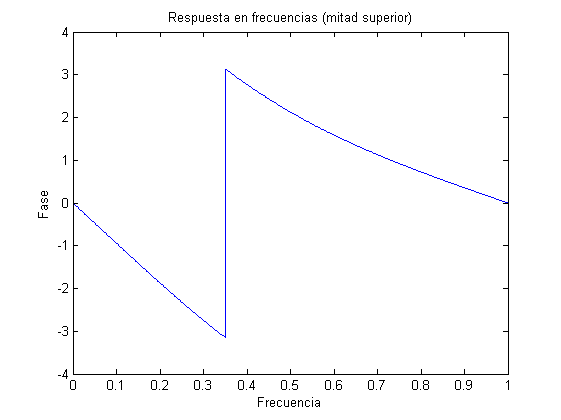
\includegraphics[width=.8 \textwidth]{ejercicio-4-6-b-fase.png}
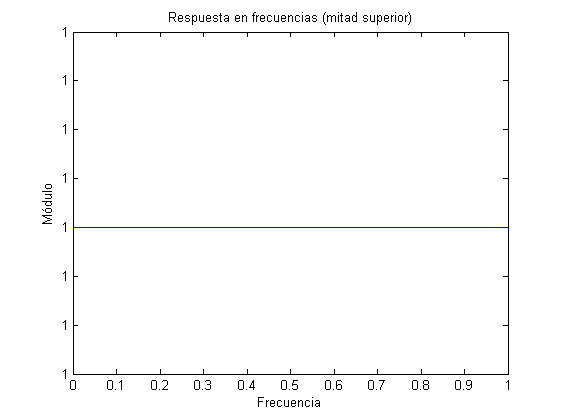
\includegraphics[width=.8 \textwidth]{ejercicio-4-6-b-modulo.png}
\end{center}

\textbf{3.c)} \\

Es un filtro pasa todo. Deja pasar todas las frecuencias y repite la señal periódicamente. \\

\lstinputlisting{ejercicio-4-6.m}

\section{Ejercicio 5}
Dados los coeficientes $a = [1 -0.8741 0.9217 0.26732]$ , \\ y $b = [0.1866 0.23360 0.23360 0.1866]$ : \\

\textbf{a)} Realice la descomposición en fracciones simples usando la función de Matlab residuez. \\

\lstinputlisting{ejercicio-5-a.m}

$$ r = -0,0428 -0,1860i; -0,0428 + 0,1860i; -0,4259 $$
$$ p = 0,5510 + 0,9323i; 0,5510 - 0,9323i; -0,2279 $$
$$ k = 0,6980 $$

Por lo que la descomposición en fracciones simples es:

\begin{eqnarray*}
H(z) & = & \frac{(-0,0428 -0,1860i)}{(1 - (0,5510 + 0,9323i) z^{-1})} + \frac{(-0,0428 + 0,1860i)}{(1 - (0,5510 - 0,9323i) z^{-1})} \\ & + & \frac{-0,4259}{(1 - (-0,2279) z^{-1})} + 0,698
\end{eqnarray*}

\textbf{b)} Calcule los polos y los ceros de la función de transferencia aplicando la función tf2zp a los coefientes proporcionados anteriormente.\\

\lstinputlisting{ejercicio-5-b.m}

Ceros: (z)\\
$$ -1,0000; -0,1259 + 0,9920i; -0,1259 - 0,9920i $$
Polos: (p)\\
$$ 0,5510 + 0,9323i; 0,5510 - 0,9323i; -0,2279 $$

Representación: \\

\begin{center}
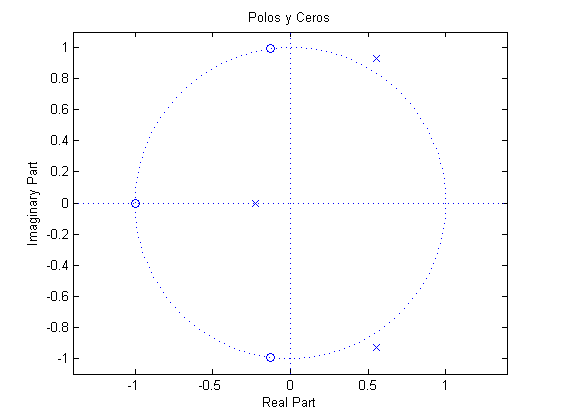
\includegraphics[width=.8 \textwidth]{ejercicio-5-b.png}
\end{center}

\textbf{c)} Calcule y dibuje 100 valores de la respuesta al impulso usando filter, y usando la expansión en fracciones simples. Compare los resultados.

Usando expansión en fracciones simples:\\
\begin{eqnarray*}
H(z) & = & \frac{(-0,0428 - 0,1860i)}{(1 - (0,5510 + 0,9323i) z^{-1})} + \frac{(-0,0428 - 0,1860i)}{(1 - (0,5510 - 0,9323i) z^{-1})} \\ & + & \frac{-0,4259}{(1 - (-0,2279) z^{-1}) + 0,698} \\ \\
y(n) & = & (-0,0428 -0,1860i)(0,5510 + 0,9323i)^n u(n) \\ & + & (-0,0428 + 0,1860i)(0,5510 - 0,9323i)^n u(n) \\ & - & 0,4259 (-0,2279)^n u(n) + 0,698 \delta(n)
\end{eqnarray*}

\begin{center}
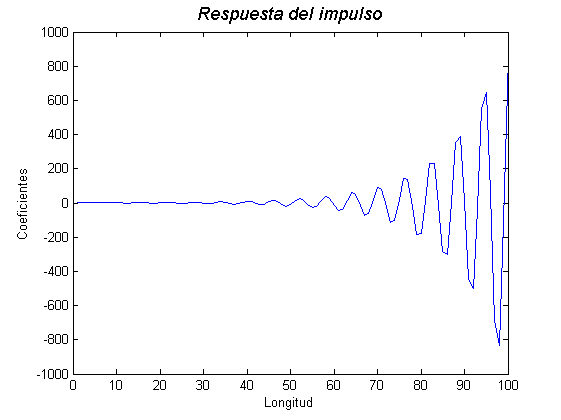
\includegraphics[width=.8 \textwidth]{ejercicio-5-c-1.png}
\end{center}

El impulso es 1 solo cuando $n$ es cero y la función es 0 en valores de tiempo negativo, por lo que la función queda como:

\[ y(n) = \left\{ 
  \begin{array}{l l}
    0 & \quad \text{si } n < 0 \\
    & \\
    (-0,0428 - 0,1860i)(0,5510 + 0,9323i)^n & \quad \\
    + (-0,0428 + 0,1860i)(0,5510 - 0,9323i)^n & \quad \\
    - 0,4259(-0,2279)^n  + 0,698 & \quad \text{si } n = 0 \\
    & \\
    (-0,0428 - 0,1860i)(0,5510 + 0,9323i)^n & \quad \\
    + (-0,0428 + 0,1860i)(0,5510 - 0,9323i)^n & \quad \\
    - 0,4259(-0,2279)^n  & \quad \text{si } n > 0
  \end{array} \right.\]

\begin{center}
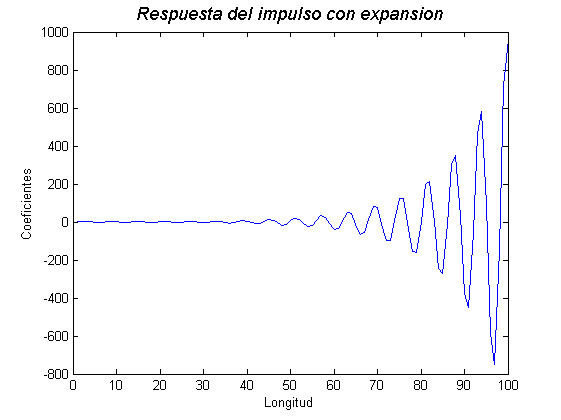
\includegraphics[width=.8 \textwidth]{ejercicio-5-c-2.png}
\end{center}

\lstinputlisting{ejercicio-5-c.m}

He realizado una función en Matlab que me calcula para cada índice desde 1 hasta 100 el valor de $y$ que hay que tomar en la representación: 

\lstinputlisting{fracciones.m}



\end{document}

